%%%%%%%%%%%%%%%%%%%%%%%%%%%%%%%%%%%%%%%%%%%%%%%%%%%%%%%%%%%%%%%%%%%%%%%%
\chapter{\appendixlabel}
%%%%%%%%%%%%%%%%%%%%%%%%%%%%%%%%%%%%%%%%%%%%%%%%%%%%%%%%%%%%%%%%%%%%%%%%
\section{Interviewleitfaden}
\label{app:leitfaden}
Als Grundlage zur Konzeption der in Kapitel \ref{sec:results} beschriebenen Teststrategie wurden Interviews mit dem leitenden Architekten der Applikation, einem Entwickler, einer Business-Analystin und einem Testverantwortlichen geführt. Das Dokument in Abbildung \ref{fig:leitfaden} diente dabei als Leitfaden.

\begin{figure}[h] 
  \centering
     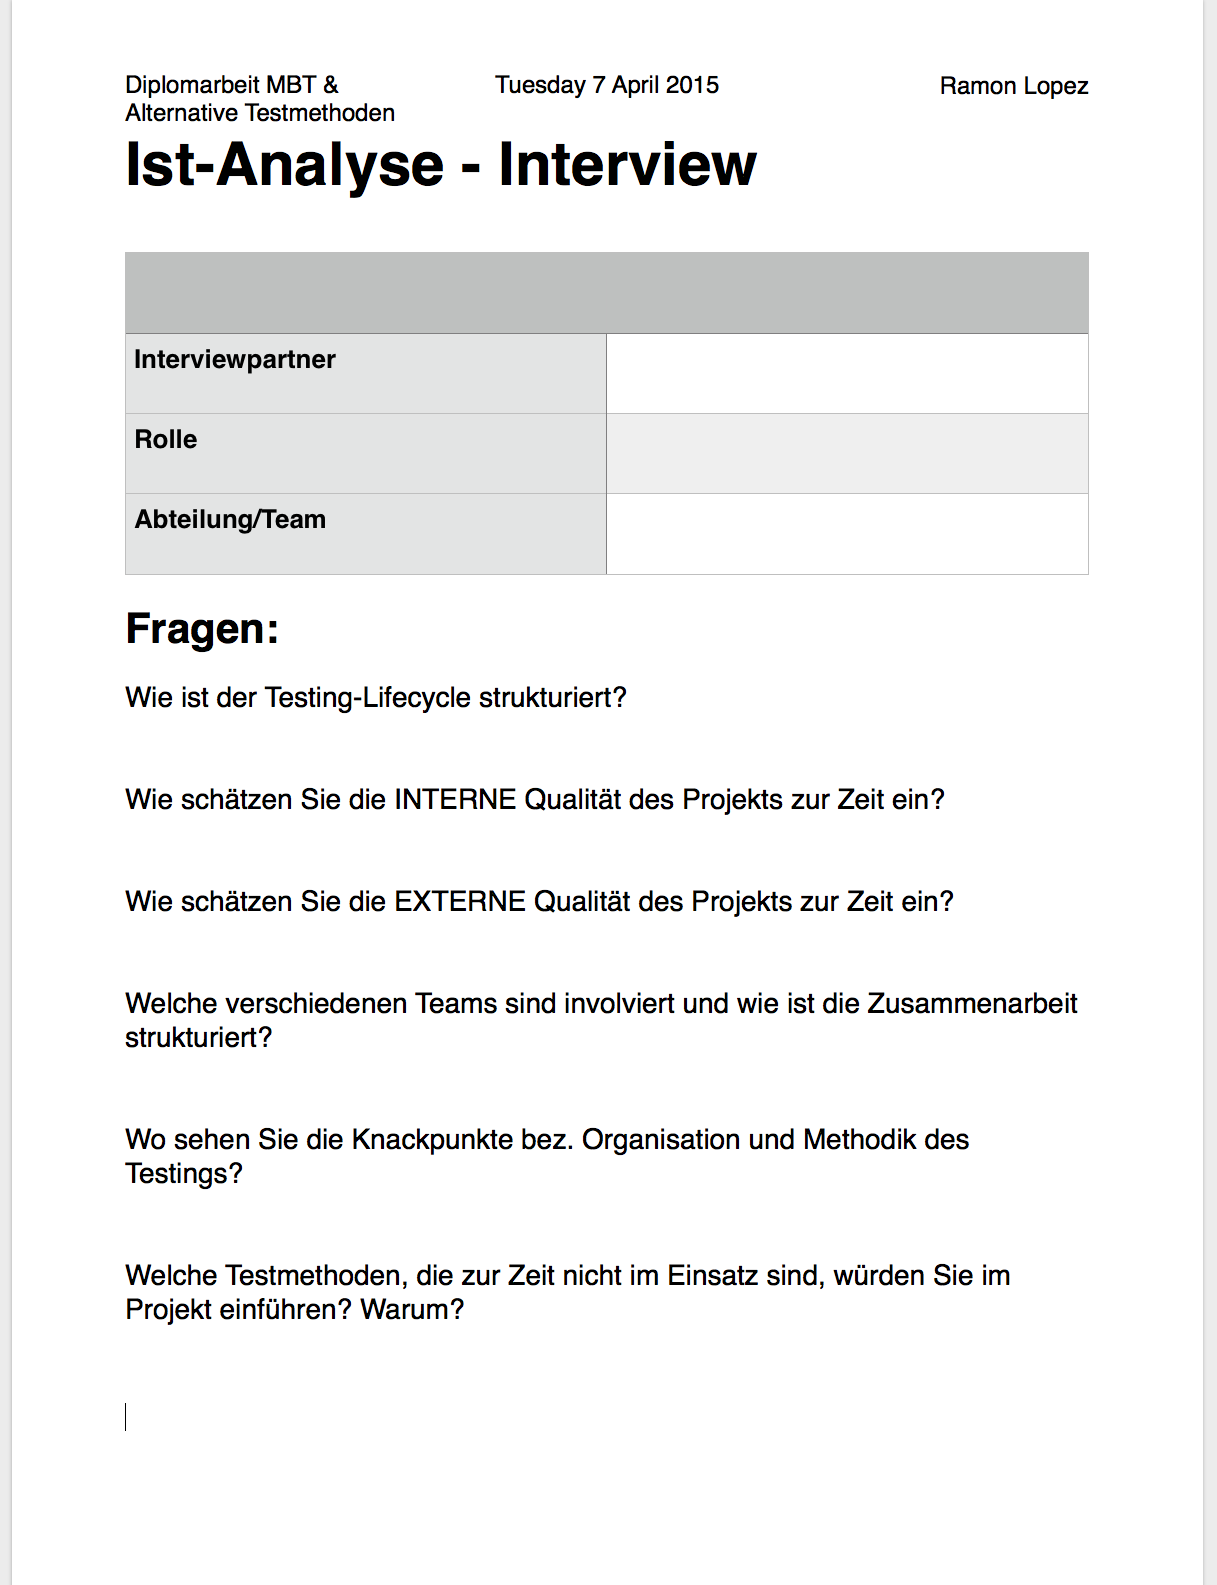
\includegraphics[width=1.0\textwidth]{figures/leitfaden.png}
  \caption{Interviewleitfadendokument}
  \label{fig:leitfaden}
\end{figure}

\section{SoapUI Testfallaufruf aus Graphwalker}
\label{app:soap}
Das folgende Beispiel \ref{code:soap_graphwalker} zeigt wie in einem Graphwalker Testfall SoapUI als Adapter-Code verwendet werden kann.\\
Die drei Methoden zum Schluss zeigen verschiedene Möglichkeiten wie Graphwalker das Testmodell traversieren kann.\\
Das vollständige Beispiel (inklusive einer vorgetäuschten REST-Schnittstelle, die der SoapUI Testfall anspricht) ist zu finden unter: \url{https://github.com/SH4DY/graphwalker-soapui/}


\begin{lstlisting}[language=Java,caption=SimpleTest.java, label=code:soap_graphwalker]
package org.myorg.testautomation;

import com.eviware.soapui.tools.SoapUITestCaseRunner;
import org.graphwalker.core.condition.EdgeCoverage;
import org.graphwalker.core.condition.ReachedVertex;
import org.graphwalker.core.condition.TimeDuration;
import org.graphwalker.core.generator.AStarPath;
import org.graphwalker.core.generator.RandomPath;
import org.graphwalker.core.machine.ExecutionContext;
import org.graphwalker.java.test.TestBuilder;
import org.junit.Test;

import java.nio.file.Path;
import java.nio.file.Paths;
import java.util.concurrent.TimeUnit;

/**
 * SoapUI 5 project running on Graphwalker
 *
 * This class represents the operations to be executed
 * when Graphwalker traverses the model. The stub generated
 * by the Graphwalker CLI is in the target directory.
 *
 * Methods prefixed with "e_" are edges, "v_" are vertices.
 *
 * The underlying model can be found at {@link SimpleTest#MODEL_PATH}
 *
 * The underlying model can be found at {@link SimpleTest#SOAPUI_PROJECT_PATH}
 * Methods in this class call according testsuites in the given project
 */
public class SimpleTest extends ExecutionContext implements Login {
    public static final Path MODEL_PATH = Paths.get("org/myorg/testautomation/Login.graphml");
    public static final String SOAPUI_PROJECT_PATH = "login/src/main/resources/soapui/GW-Test-Project-soapui-project.xml";

    @Override
    public void e_InvalidCredentials() {

        //Try login with invalid credentials
        SoapUITestCaseRunner runner = new SoapUITestCaseRunner();
        runner.setProjectFile(SOAPUI_PROJECT_PATH);
        runner.setTestSuite("InvalidLogin");
        try {
            runner.run();
        } catch (Exception e) {
            e.printStackTrace();
        }
    }

    @Override
    public void e_ValidCredentials() {

        //Invoke SoapUI testcase with valid credentials
        SoapUITestCaseRunner runner = new SoapUITestCaseRunner();
        runner.setProjectFile(SOAPUI_PROJECT_PATH);
        runner.setTestSuite("ValidLogin");
        try {
            runner.run();
        } catch (Exception e) {
            e.printStackTrace();
        }
    }

    //All the other edges and nodes have to be overriden as well

    @Test
    public void runSmokeTest() {
        new TestBuilder()
                .setModel(MODEL_PATH)
                .setContext(new SimpleTest())
                .setPathGenerator(new AStarPath(new ReachedVertex("v_Browse")))
                .setStart("e_Init")
                .execute();
    }

    @Test
    public void runFunctionalTest() {
        new TestBuilder()
                .setModel(MODEL_PATH)
                .setContext(new SimpleTest())
                .setPathGenerator(new RandomPath(new EdgeCoverage(100)))
                .setStart("e_Init")
                .execute();
    }

    //@Test
    public void runStabilityTest() {
        new TestBuilder()
                .setModel(MODEL_PATH)
                .setContext(new SimpleTest())
                .setPathGenerator(new RandomPath(new TimeDuration(30, TimeUnit.SECONDS)))
                .setStart("e_Init")
                .execute();
    }

}
\end{lstlisting}


\section{Graphwalker Testsuite am Beispiel Hypothekarrechner mit Selenium}
Es folgt der Code zum Beispiel aus Kapitel \ref{sec:results} - \Newnameref{sec:results}. Hier wird das \Gls{SUT} im GraphML-Format dargestellt. Graphwalker erzeugt ein Java Interface, welches der Testentwickler mit Adapter-Code befüllt. In diesem Beispiel wurde Selenium verwendet um die Applikation anzusteuern.\\

Das Codebeispiel \ref{code:gw_generated} zeigt das von Graphwalker generierte Java Interface. Wie das zugrundeliegende Modell \ref{fig:modell_logisch} erstellt wurde, wird im Abschnitt \ref{sec:results_modellierung} beschrieben.\\

Im Listing \ref{code:gw_selenium} wird das generierte Interface implementiert. Nicht alle Knoten und Kanten müssen Adapter-Code enthalten.\\

Das vollständige Beispiel, inklusive der generierten GraphML-Dateien, ist zu finden unter: \url{https://github.com/SH4DY/ImexTest/}

\begin{lstlisting}[language=Java,caption=ImexTest.java, label=code:gw_selenium]
package com.shady.imextest.modelimplementations;

import com.shady.imextest.ModellLogisch;
import org.graphwalker.core.condition.EdgeCoverage;
import org.graphwalker.core.condition.ReachedVertex;
import org.graphwalker.core.generator.AStarPath;
import org.graphwalker.core.generator.RandomPath;
import org.graphwalker.core.machine.ExecutionContext;
import org.graphwalker.java.annotation.GraphWalker;
import org.graphwalker.java.test.Result;
import org.graphwalker.java.test.TestBuilder;
import org.junit.Assert;
import org.junit.Test;
import org.openqa.selenium.*;
import org.openqa.selenium.chrome.ChromeDriver;
import org.openqa.selenium.support.ui.*;

import java.nio.file.Path;
import java.nio.file.Paths;
import java.util.concurrent.TimeUnit;

/**
 * Diese Klasse beinhaltet alle Kanten und Knoten aus dem entsprechenden logischen Modell des
 * Hypothekarrechners. Im Modell sind es 51 Knoten und 66 Kanten. Im Code sind es aber deutlich
 * weniger Methoden.
 *
 */
@GraphWalker(value = "random(edge_coverage(100))", start = "e_init")
public class ImexTest extends ExecutionContext implements ModellLogisch {

    private final static Path MODEL_PATH = Paths.get("com/shady/imextest/ModellLogisch.graphml");
    private WebDriver driver;

    private final String HYPO_URL= "https://www.raiffeisen.ch/rch/de/privatkunden/hypotheken/wohneigentum-kaufen/wieviel-eigenheim-kann-ich-mir-leisten.html";

//    @Test
//    public void runSmokeTest() {
//        TestBuilder tb = new TestBuilder()
//                .addModel(MODEL_PATH,
//                        new ImexTest().setPathGenerator(new AStarPath(new ReachedVertex("v_Proposal_7_Libor"))));
//
//        Result result = tb.execute();
//        System.out.println("Done: [" + result.getErrors().toString() + "," + result.getFailedCount() + "]");
//    }

    @Test
    public void runFunctionalTest() {
                TestBuilder tb = new TestBuilder()
                        .addModel(MODEL_PATH,
                                new ImexTest().setPathGenerator(new RandomPath(new EdgeCoverage(100))));
        Result result = tb.execute();
        System.out.println("Done: [" + result.getErrors().toString() + "," + result.getFailedCount() + "]");

    }
//
//    @Test
//    public void runStabilityTest() {
//        new TestBuilder()
//                .setModel(MODEL_PATH)
//                .setContext(new ImexTest())
//                .setPathGenerator(new RandomPath(new TimeDuration(30, TimeUnit.SECONDS)))
//                .setStart("e_Init")
//                .execute();
//    }

    @Override
    public void e_init() {
        driver = new ChromeDriver();

        //Selenium wartet somit 10 Sek. bevor eine NotFound exception geworfen wird.
        driver.manage().timeouts().implicitlyWait(10, TimeUnit.SECONDS);
    }


    @Override
    public void v_OnPage() {
        driver.get(HYPO_URL);
    }


    @Override
    public void v_PLZPrompt() {
    }

    @Override
    public void e_EnterPLZ() {
        WebElement searchBox = driver.findElement(By.className("dropdown-toggle"));
        searchBox.sendKeys("6900");

        WebDriverWait wait = new WebDriverWait(driver, 10);
        wait.until(ExpectedConditions.elementToBeClickable(By.partialLinkText("Lugano")));

        driver.findElement(By.partialLinkText("Lugano")).click();

    }

    @Override
    public void v_Wieviel() {
    }

    @Override
    public void e_EnterCredibility() {

        Wait wait = new FluentWait<WebDriver>(driver)
                .withTimeout(5, TimeUnit.SECONDS)
                .pollingEvery(500, TimeUnit.MILLISECONDS)
                .ignoring(WebDriverException.class);

        wait.until(ExpectedConditions.elementToBeClickable(By.id("financingObject.initialCost")));

        driver.findElement(By.id("financingObject.initialCost")).clear();
        driver.findElement(By.id("financingObject.initialCost")).sendKeys("500000");

        try {
            Thread.sleep(3000);
        } catch (InterruptedException e) {
            e.printStackTrace();
        }

        driver.findElement(By.xpath("//*[@id=\"maincontent\"]/div/div/div[3]/div[3]/div/div[2]/a")).click();
    }

    @Override
    public void e_ClickStartProposal() {
        try {
            Thread.sleep(2000);
        } catch (InterruptedException e) {
            e.printStackTrace();
        }
        driver.findElement(By.cssSelector("body > div.perspective > div.viewport > div.parbase.consultantflyin > div > div > div > div.content.ng-scope > div > div.par.parsys > div.parbase.linkbutton.section > a")).click();
    }

    @Override
    public void e_ClickUnwichtig() {
        driver.findElement(By.linkText("unwichtig")).click();
    }

    @Override
    public void e_ClickWichtig() {
        driver.findElement(By.linkText("wichtig")).click();
    }

    @Override
    public void e_ClickSehrWichtig() {
        driver.findElement(By.linkText("sehr wichtig")).click();
    }

    @Override
    public void e_ClickSinkend() {
        driver.findElement(By.linkText("sinkend")).click();
    }

    @Override
    public void e_ClickGleichbleibend() {
        driver.findElement(By.linkText("gleichbleibend")).click();
    }

    @Override
    public void e_ClickSteigend() {
        driver.findElement(By.linkText("steigend")).click();
    }

    @Override
    public void e_ClickAusgabenJa() {
        driver.findElement(By.linkText("ja")).click();
    }
    @Override
    public void e_ClickAusgabenNein() {
        driver.findElement(By.linkText("nein")).click();
    }

    @Override
    public void e_ClickPersoenlichJa() {
        driver.findElement(By.linkText("ja")).click();
    }

    @Override
    public void e_ClickPersoenlichNein() {
        driver.findElement(By.linkText("nein")).click();
    }

    /*
    Die folgenden Knoten repraesentieren die Endzustaende. Mit dieser Art
    der Modellierung muss in ihnen nur sehr wenig Code fuer Ueberpruefungen
    untergebracht werden.
     */
    @Override
    public void v_Proposal_0() {

        //Beispielsweise
        Assert.assertTrue(driver.findElement(
                By.xpath("//*[@id=\"maincontent\"]/div/div/div[3]/div[2]/div/div[2]/div[2]/div/table[1]/thead/tr/th[1]"))
                .getText()
                .equals("Festhypothek"));
    }

    //Weitere Blattknoten in denen Ueberpruefungen stattfinden...
\end{lstlisting}

\begin{lstlisting}[language=Java,caption=ModellLogisch.java, label=code:gw_generated]
package com.shady.imextest;

import org.graphwalker.java.annotation.Model;
import org.graphwalker.java.annotation.Vertex;
import org.graphwalker.java.annotation.Edge;

@Model(file = "com/shady/imextest/ModellLogisch.graphml")
public interface ModellLogisch {

    @Vertex()
    void v_Proposal_5_Libor();

    @Vertex()
    void v_Proposal_8();

    @Edge()
    void e_EnterCredibility();

    @Vertex()
    void v_Zinsentwicklung();

    @Vertex()
    void v_Proposal_5();

    @Vertex()
    void v_Proposal_4();

    @Vertex()
    void v_Proposal_7();

    @Vertex()
    void v_Proposal_6();

    @Vertex()
    void v_Wieviel();

    @Edge()
    void e_ClickUnwichtig();

    @Edge()
    void e_ClickSteigend();

    @Vertex()
    void v_Proposal_0_Libor();

    @Vertex()
    void v_ZinsentwicklungPersoenlich();

    @Vertex()
    void v_PLZPrompt();

    @Edge()
    void e_ClickWichtig();

    @Vertex()
    void v_Proposal_8_Libor();

    @Vertex()
    void v_Proposal_1_Libor();

    @Edge()
    void e_ClickStartProposal();

    @Vertex()
    void v_Proposal();

    @Vertex()
    void v_Proposal_3_Libor();

    @Vertex()
    void v_Proposal_1();

    @Vertex()
    void v_Proposal_0();

    @Vertex()
    void v_Proposal_3();

    @Vertex()
    void v_Proposal_6_Libor();

    @Edge()
    void e_ClickSinkend();

    @Edge()
    void e_ClickGleichbleibend();

    @Vertex()
    void v_Proposal_2();

    @Vertex()
    void v_Ausgaben();

    @Vertex()
    void v_OnPage();

    @Edge()
    void e_ClickSehrWichtig();

    @Vertex()
    void v_Proposal_4_Libor();

    @Edge()
    void e_ClickAusgabenJa();

    @Edge()
    void e_ClickPersoenlichNein();

    @Edge()
    void e_init();

    @Edge()
    void e_ClickPersoenlichJa();

    @Edge()
    void e_EnterPLZ();

    @Vertex()
    void v_Proposal_7_Libor();

    @Vertex()
    void v_PlanbareKosten();

    @Edge()
    void e_ClickAusgabenNein();

    @Vertex()
    void v_Proposal_2_Libor();
}
\end{lstlisting}

\section{Beispielhaftes BDD Framework: FluentCoS}
\label{app:fluent}
FluentCoS zeigt eine mögliche Implementierung eines einfachen BDD Frameworks. Es findet keine Übersetzung zwischen Klartext Testfalldefinitionen und Code statt. Wie in Kapitel \ref{sec:testing_api} beschrieben, würden innerhalb der folgenden Testfälle die Methoden verwendet werden, die die Testing API anbietet.\\

Codebeispiel \ref{code:fluent} zeigt die Implementierung des Frameworks an sich. Beispiel \ref{code:fluent_demand} zeigt exemplarisch wie eine \Gls{COS} in einen BDD Testfall umgesetzt wird. Um \Gls{COS} Dokumente mit funktionalen Testfällen zu verbinden wird als Datei- und Klassennamen per Konvention der Name der \Gls{COS} gewählt.\\

Das vollständige Beispiel ist zu finden unter: \url{https://github.com/SH4DY/FluentCoS/}

\begin{lstlisting}[language=Java,caption=FluentCos.java, label=code:fluent]
package ch.raiffeisen.fluentcos;

import static org.junit.Assert.fail;


public final class FluentCos {
	
	public static boolean nop() {
		return true;
	}
	
	private FluentCos() {
		// Toolsklasse
	}
	
	public static Given given(String text, boolean mapped) {
		System.out.println();
		return new Given("given: ", text, mapped);
	}
	
	public static Given given(String text) {
		return given(text, false);
	}
	
	public static class Given {
		private Given(String prefix, String text, boolean mapped) {
			System.out.println(prefix + text);
			if (!mapped) {
				fail("The statement '" + prefix + text + "' is not mapped.");
			}
		}
		
		public Given and(String text) {
			return and(text, false);
		}
		
		public Given and(String text, boolean mapped) {
			return new Given("    and: ", text, mapped);
		}
		
		public When when(String text) {
			return when(text, false);
		}
		
		public When when(String text, boolean mapped) {
			return new When("  when: ", text, mapped);
		}
	}
	
	public static class When {
		private When(String prefix, String text, boolean mapped) {
			System.out.println(prefix + text);
			if (!mapped) {
				fail("The statement '" + prefix + text + "' is not mapped.");
			}
		}
		
		public When and(String text) {
			return and(text, false);
		}
		
		public When and(String text, boolean mapped) {
			return new When("    and: ", text, mapped);
		}
		
		public Then then(String text) {
			return then(text, false);
		}
		
		public Then then(String text, boolean mapped) {
			return new Then("  then: ", text, mapped);
		}
	}
	
	public static class Then {
		private Then(String prefix, String text, boolean mapped) {
			System.out.println(prefix + text);
			if (!mapped) {
				fail("The statement '" + prefix + text + "' is not mapped.");
			}
		}
		
		public Then and(String text) {
			return and(text, false);
		}
		
		public Then and(String text, boolean mapped) {
			return new Then("    and: ", text, mapped);
		}
	}
}

\end{lstlisting}

\begin{lstlisting}[language=Java,caption=Demand111958.java, label=code:fluent_demand]


package ch.raiffeisen.casi.tests.ffox;

import static ch.raiffeisen.fluentcos.FluentCos.given;
import static ch.raiffeisen.fluentcos.FluentCos.nop;
import static org.junit.Assert.assertEquals;
import static org.junit.Assert.assertNotEquals;

import java.util.*;

import org.junit.Ignore;
import org.junit.Test;

/**
 * Conditions of Satisfaction fuer Demand_111958_FFOX_ANL_Migration des
 * Anlageziels auf TV Spar- und Vorsorgevermoegen
 * 
 * @author Damian Hofmann <damian.hofmann@raiffeisen.ch>
 */
public class Demand111958_MigrationDesAnlagezielsAufTvSparvermoegenUndVorsorgevermoegen {

	/**
	 * Es muss fachlich sichergestellt sein, dass ...
	 * Lorem Ipsum
	 */
	@Test
	public final void coc_1_Hierarchische_Auflistung_und_Bezeichnung_des_Default_Teilvermoegens_Kontovermoegen() {
			given("Kunde XY fuer Beratung ausgewaehlt", selectCustomer("Peter Mueller"))
				.and("Kunde XY besitzt Produkte des TV's 'Kontovermoegen'", initCustomerAssets())
			.when("Berater fuer Kunde XY den Menuepunkt 'Anlegen Finfox' anklickt", clickMenu())
			.then("Wird das TV 'Kontovermoegen' an erster Stelle gezeigt", assertAccountFirst())
				.and("Der Titel des TV beinhaltet eine eindeutige Nummer", assertUniquePortfolioId())
				.and("Den TV-Typ 'Kontovermoegen'", nop());
	}
		
	
	/**
	 * Es muss fachlich sichergestellt sein, dass ...
	 */
	@Ignore // Future CoS. Planned for Sprint 4264324532
	@Test
	public final void cos_2_Hierarchische_Auflistung_und_Bezeichnung_des_Default_Teilvermoegens_Anlagevermoegen() {
			given("Kunde XY fuer Beratung ausgewaehlt")
				.and("Kunde XY besitzt Produkte des TV's 'Anlagevermoegen'")
			.when("Berater fuer Kunde XY den Menuepunkt 'Anlegen Finfox' anklickt")
			.then("Wird das TV 'Anlagevermoegen' an zweiter Stelle gezeigt")
				.and("Der Titel des TV beinhaltet eine eindeutige Nummer")
				.and("Den TV-Typ 'Anlagevermoegen'");
	}
	
	/*
	 * Everything below this line belongs to the developers
	 */
	
	private  boolean selectCustomer(String name) {
		customer = new Customer();
		customer.name = name;
		return true;
	}

	private boolean initCustomerAssets() {
		customerAssets = new LinkedList<Asset>();
		customerAssets.add(createAsset("Peter Mueller", "Vorsorgekonto", "provision"));
		customerAssets.add(createAsset("Peter Mueller", "Sparkonto", "account"));
		customerAssets.add(createAsset("Karolina Cantieni", "Fonssparkonto", "invest"));
		return true;
	}

	private Asset createAsset(String customer, String name, String type) {
		Asset asset = new Asset();
		asset.customer = customer;
		asset.name = name;
		asset.type = type;
		return asset;
	}

	private boolean clickMenu() {
		portfolios = customerAdvisoryDataServerGetPortfolios(customer);
		return true;
	}

	private boolean assertAccountFirst() {
		Portfolio portfolio = portfolios.get(0);
		assertEquals("account", portfolio.type);
		return true;
	}

	private boolean assertUniquePortfolioId() {
		int id = portfolios.get(0).id;
		for (int i=1; i<portfolios.size(); i++) {
			assertNotEquals(id, portfolios.get(i).id);
		}
		return true;
	}
	
	/*
	 * Just a few dummy models for this showcase.
	 */
	
	private List<Portfolio> customerAdvisoryDataServerGetPortfolios(Customer customer) {
		Set<String> portfolioTypes = new HashSet<String>();
		for (Asset asset : customerAssets) {
			if (!asset.customer.equals(customer.name)) {
				continue;
			}
			
			portfolioTypes.add(asset.type);
		}
		
		List<Portfolio> portfolios = new ArrayList<Portfolio>();
		for (String portfolioType : portfolioTypes) {
			Portfolio portfolio = new Portfolio();
			portfolio.id = new Random().nextInt();
			portfolio.name = "Teilvermoegen";
			portfolio.type = portfolioType;
			portfolios.add(portfolio);
		}
		return portfolios;
	}
	
	private Customer customer;
	private List<Asset> customerAssets = new ArrayList<Asset>();
	private List<Portfolio> portfolios;
	
	private static class Customer {
		private String name;
	}
	
	private static class Asset {
		private String customer;
		private String name;
		private String type;
	}
	
	private static class Portfolio {
		private int id;
		private String name;
		private String type;
	}
}
\end{lstlisting}















